\documentclass{article}
\usepackage[dvipsnames]{xcolor}
\usepackage[paperwidth=10cm, paperheight=2.5cm, margin = 0cm, top=0.25cm]{geometry}
\usepackage{amsmath}


\usepackage{pgf}
\usepackage{tikz}
\usetikzlibrary{positioning, calc}
\usetikzlibrary{arrows,automata}



\renewcommand{\vec}[1]{\boldsymbol{#1}}

\begin{document}
\begin{center}
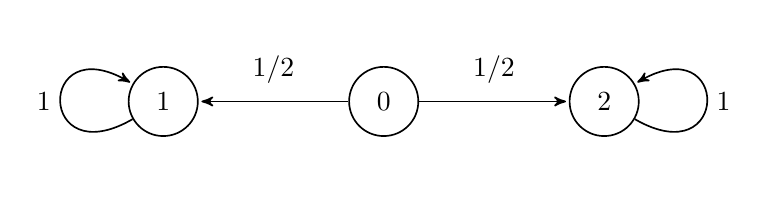
\begin{tikzpicture}[->,>=stealth',shorten >=1pt,auto,node distance=2.8cm,semithick]
                    
\node[state] (X0)                             {$0$}; 
\node[state] (X1) [left of=X0, yshift=+0.0cm] {$1$};
\node[state] (X2) [right of=X0, yshift=-0.0cm]{$2$};
\path
	(X0) edge[bend right=0] node[above, yshift=+0.1cm]{$1/2$} (X1)
	(X0) edge[bend left=0]  node[above, yshift=+0.1cm]{$1/2$} (X2);
\path	
	(X1) edge[in=150, out=210, looseness=7, loop, left]  node[left]{$1$} (X1)
	(X2) edge[in=30,  out=-30, looseness=7, loop, right] node[right]{$1$} (X2);
\end{tikzpicture}
\end{center}

\end{document}
